% ============================================================
% PORTFOLIO
% Shamekh Al-Suwi
% Compiler: pdfLaTeX
% ============================================================

\documentclass[10pt,a4paper]{article}

\usepackage[margin=1.9cm]{geometry}
\usepackage[T1]{fontenc}
\usepackage[utf8]{inputenc}
\usepackage[scaled=0.94]{helvet}
\renewcommand{\familydefault}{\sfdefault}
\usepackage{microtype}
\usepackage{graphicx}
\usepackage{xcolor}
\usepackage{fancyhdr}
\usepackage{lastpage}
\usepackage[colorlinks=true,urlcolor=accent,linkcolor=accent]{hyperref}

\definecolor{ink}{HTML}{1B1B1B}
\definecolor{muted}{HTML}{6A6A6A}
\definecolor{accent}{HTML}{0E6B62}
\definecolor{line}{HTML}{D9D3C7}

\setlength{\parindent}{0pt}
\setlength{\parskip}{0pt}

% Running footer
\pagestyle{fancy}
\fancyhf{}
\renewcommand{\headrulewidth}{0pt}
\renewcommand{\footrulewidth}{0.3pt}
\fancyfoot[L]{\footnotesize\color{muted}Shamekh Al-Suwi \textperiodcentered\ Portfolio}
\fancyfoot[R]{\footnotesize\color{muted}\thepage\ of \pageref{LastPage}}

% Project block
\newenvironment{proj}[2]{%
  \par
  {\large\bfseries\color{ink}#1}\hfill{\footnotesize\href{#2}{\color{accent}Repository}}\par\vspace{3pt}%
}{\par\vspace{16pt}}

% Stack line
\newcommand{\stack}[1]{{\footnotesize\color{muted}\textsc{Stack}\enspace #1}\par}

% Framed, centered screenshot
\newcommand{\shot}[2]{%
  \IfFileExists{#1}{%
    \par\vspace{6pt}%
    \begin{center}%
      {\setlength{\fboxrule}{0.4pt}\setlength{\fboxsep}{3pt}%
       \fcolorbox{line}{white}{\includegraphics[width=#2\linewidth]{#1}}}%
    \end{center}%
    \par\vspace{2pt}%
  }{}%
}

\newcommand{\diag}[2]{%
  \IfFileExists{#1}{%
    \par\vspace{7pt}%
    \begin{center}{\setlength{\fboxrule}{0.4pt}\setlength{\fboxsep}{3pt}\fcolorbox{line}{white}{\includegraphics[width=#2\linewidth]{#1}}}\end{center}%
    {\centering\footnotesize\color{muted}Architecture\par}\vspace{1pt}%
  }{}%
}

\begin{document}

\begin{center}
  {\fontsize{30}{34}\selectfont\bfseries Portfolio}\\[4pt]
  {\Large Shamekh Al-Suwi}
\end{center}

\vspace{2pt}
{\color{accent}\rule{\linewidth}{1.4pt}}
\vspace{12pt}

%------------------------------------------------------------
\begin{proj}{cfd-sim}{https://github.com/shamekhing/cfd-sim}
A computational fluid dynamics engine written from scratch. It simulates air
flowing around a cylinder by solving the incompressible Navier-Stokes equations
on a staggered grid with the SIMPLE algorithm, and it reproduces the
K\'arm\'an vortex street behind the cylinder. Optional CUDA acceleration.

\vspace{5pt}
\stack{C++17, CUDA, Numerical Methods}
\shot{img/cfd-sim.png}{0.8}
\diag{img/mmd-cfd-sim.png}{0.95}

\end{proj}

%------------------------------------------------------------
\begin{proj}{cv\_deepSort}{https://github.com/shamekhing/cv\_deepSort}
A multi-object tracking pipeline for video. YOLOv5 detects objects in each frame
and Deep SORT keeps a stable identity on each one by combining motion prediction
with appearance embeddings. Built for drone footage, with recorded result clips.

\vspace{5pt}
\stack{Python, PyTorch, OpenCV}
\shot{img/cv_deepSort.png}{0.55}
\diag{img/mmd-cv_deepSort.png}{0.95}

\end{proj}

%------------------------------------------------------------
\begin{proj}{OpenJoey2}{https://github.com/shamekhing/OpenJoey2}
A Yu-Gi-Oh! engine that implements the classic ruleset from scratch in C++17:
summon types, attack and defense math, chains with Spell Speeds, and bounded
undo snapshots. A raylib interface drives the game, and the same code builds for
the browser.

\vspace{5pt}
\stack{C++17, Raylib, Game Engine}
\shot{img/openjoey2.png}{0.8}
\diag{img/mmd-OpenJoey2.png}{0.95}

\end{proj}

%------------------------------------------------------------
\begin{proj}{doomai}{https://github.com/shamekhing/doomai}
Reinforcement learning agents for the JKU ViZDoom deathmatch challenge. Each
agent first learns by imitating recorded human play, then improves with PPO and
DQN training rewarded for frags, and exports to ONNX.

\vspace{5pt}
\stack{Python, PyTorch, RL}
\shot{img/doomai.png}{0.4}
\diag{img/mmd-doomai.png}{0.95}

\end{proj}

%------------------------------------------------------------
\begin{proj}{fpga-snn}{https://github.com/shamekhing/fpga-snn}
An experimental spiking neural network accelerator for MNIST, where neurons carry
information as spike timing instead of numbers. A Python trainer learns the
weights and a SystemVerilog datapath replays them on a Gowin FPGA.

\vspace{5pt}
\stack{SystemVerilog, Python, SNN}
\shot{img/fpga-snn.png}{0.85}
\diag{img/mmd-fpga-snn.png}{0.95}

\end{proj}

%------------------------------------------------------------
\begin{proj}{Ahoy}{https://github.com/shamekhing/Ahoy}
A privacy-first messaging app in Flutter for phones that are near each other. It
picks the best direct link (Wi-Fi Direct, LAN or Bluetooth), encrypts messages
end to end so keys never leave the phone, and needs no server or account.

\vspace{5pt}
\stack{Dart, Flutter, Privacy}

\par\vspace{8pt}
\begin{center}
  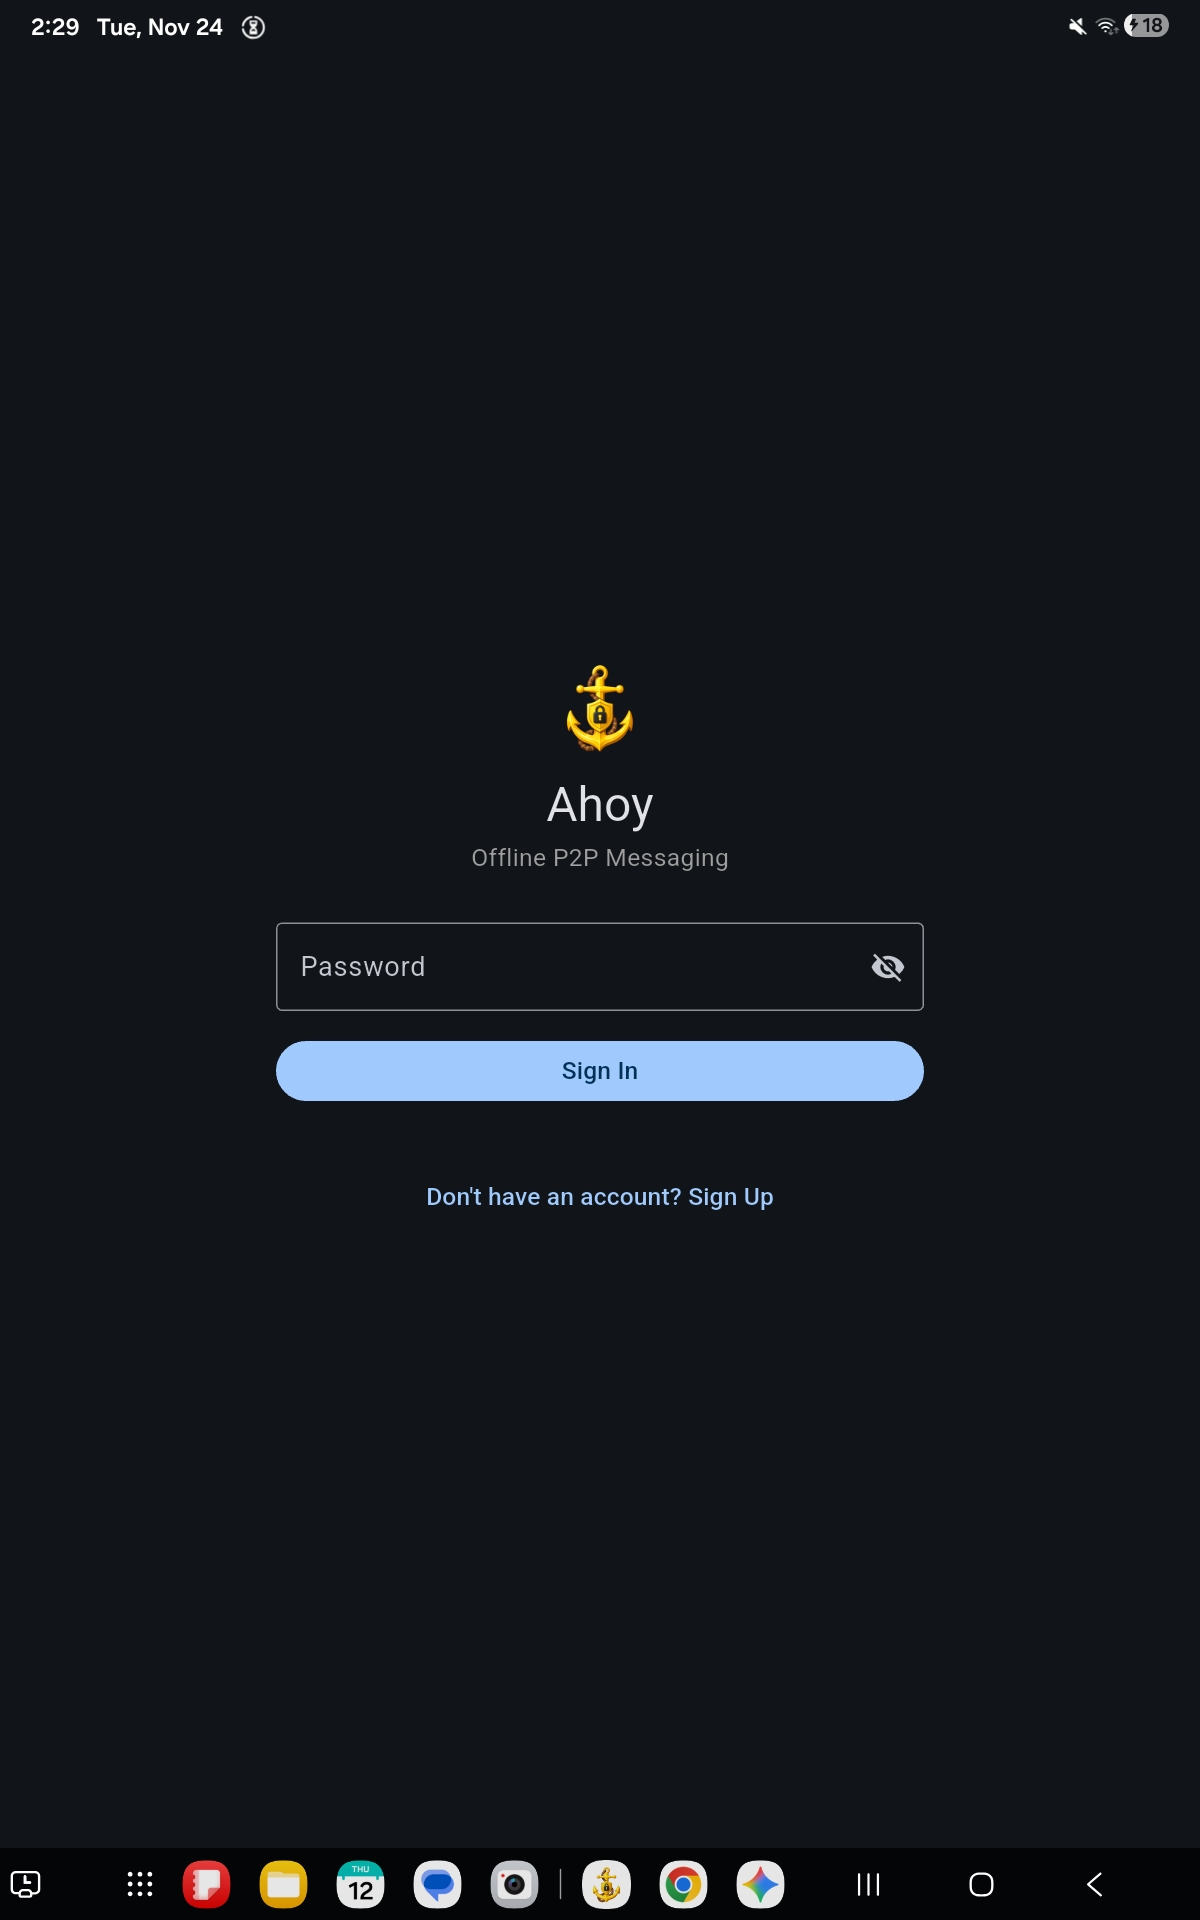
\includegraphics[width=0.175\linewidth]{img/ahoy-1.jpg}\hfill
  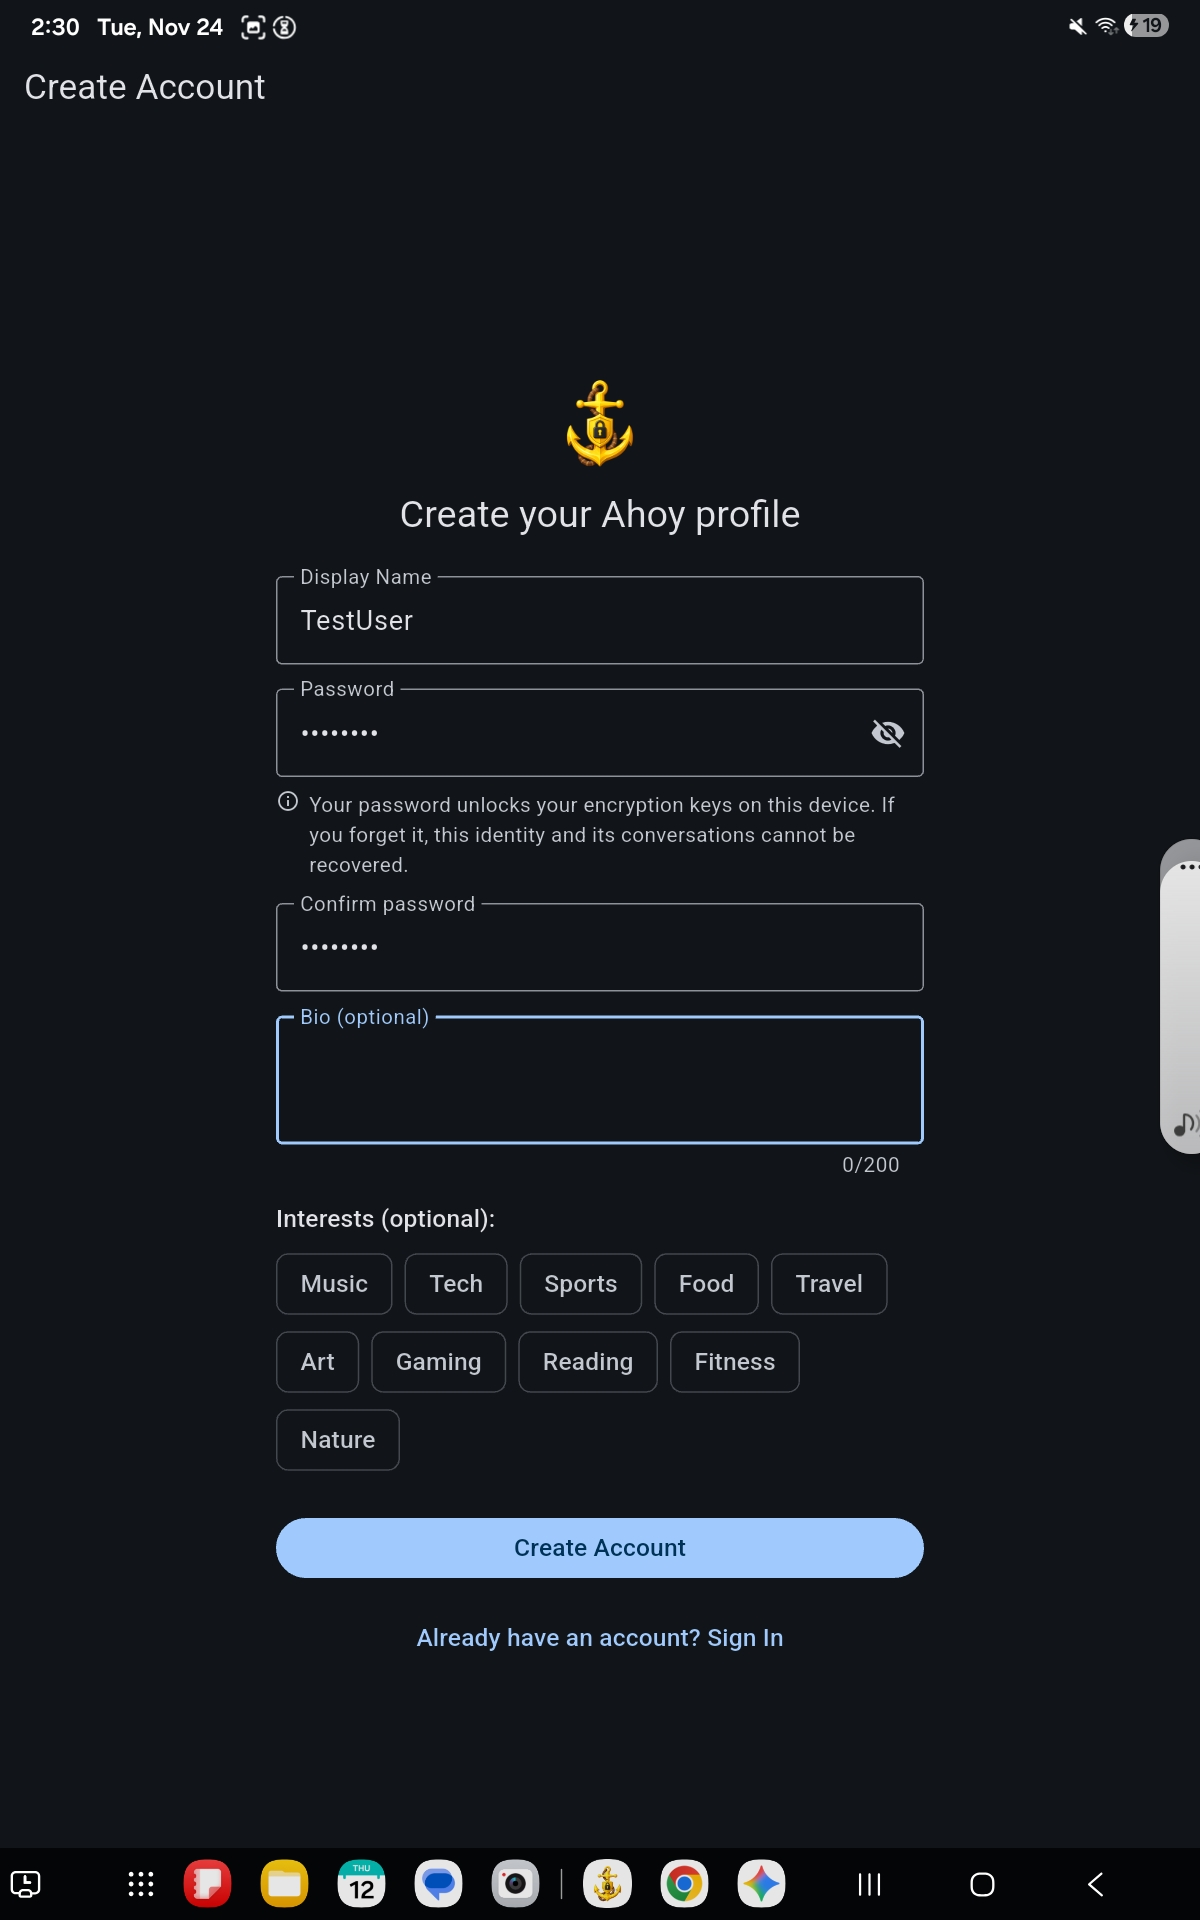
\includegraphics[width=0.175\linewidth]{img/ahoy-2.jpg}\hfill
  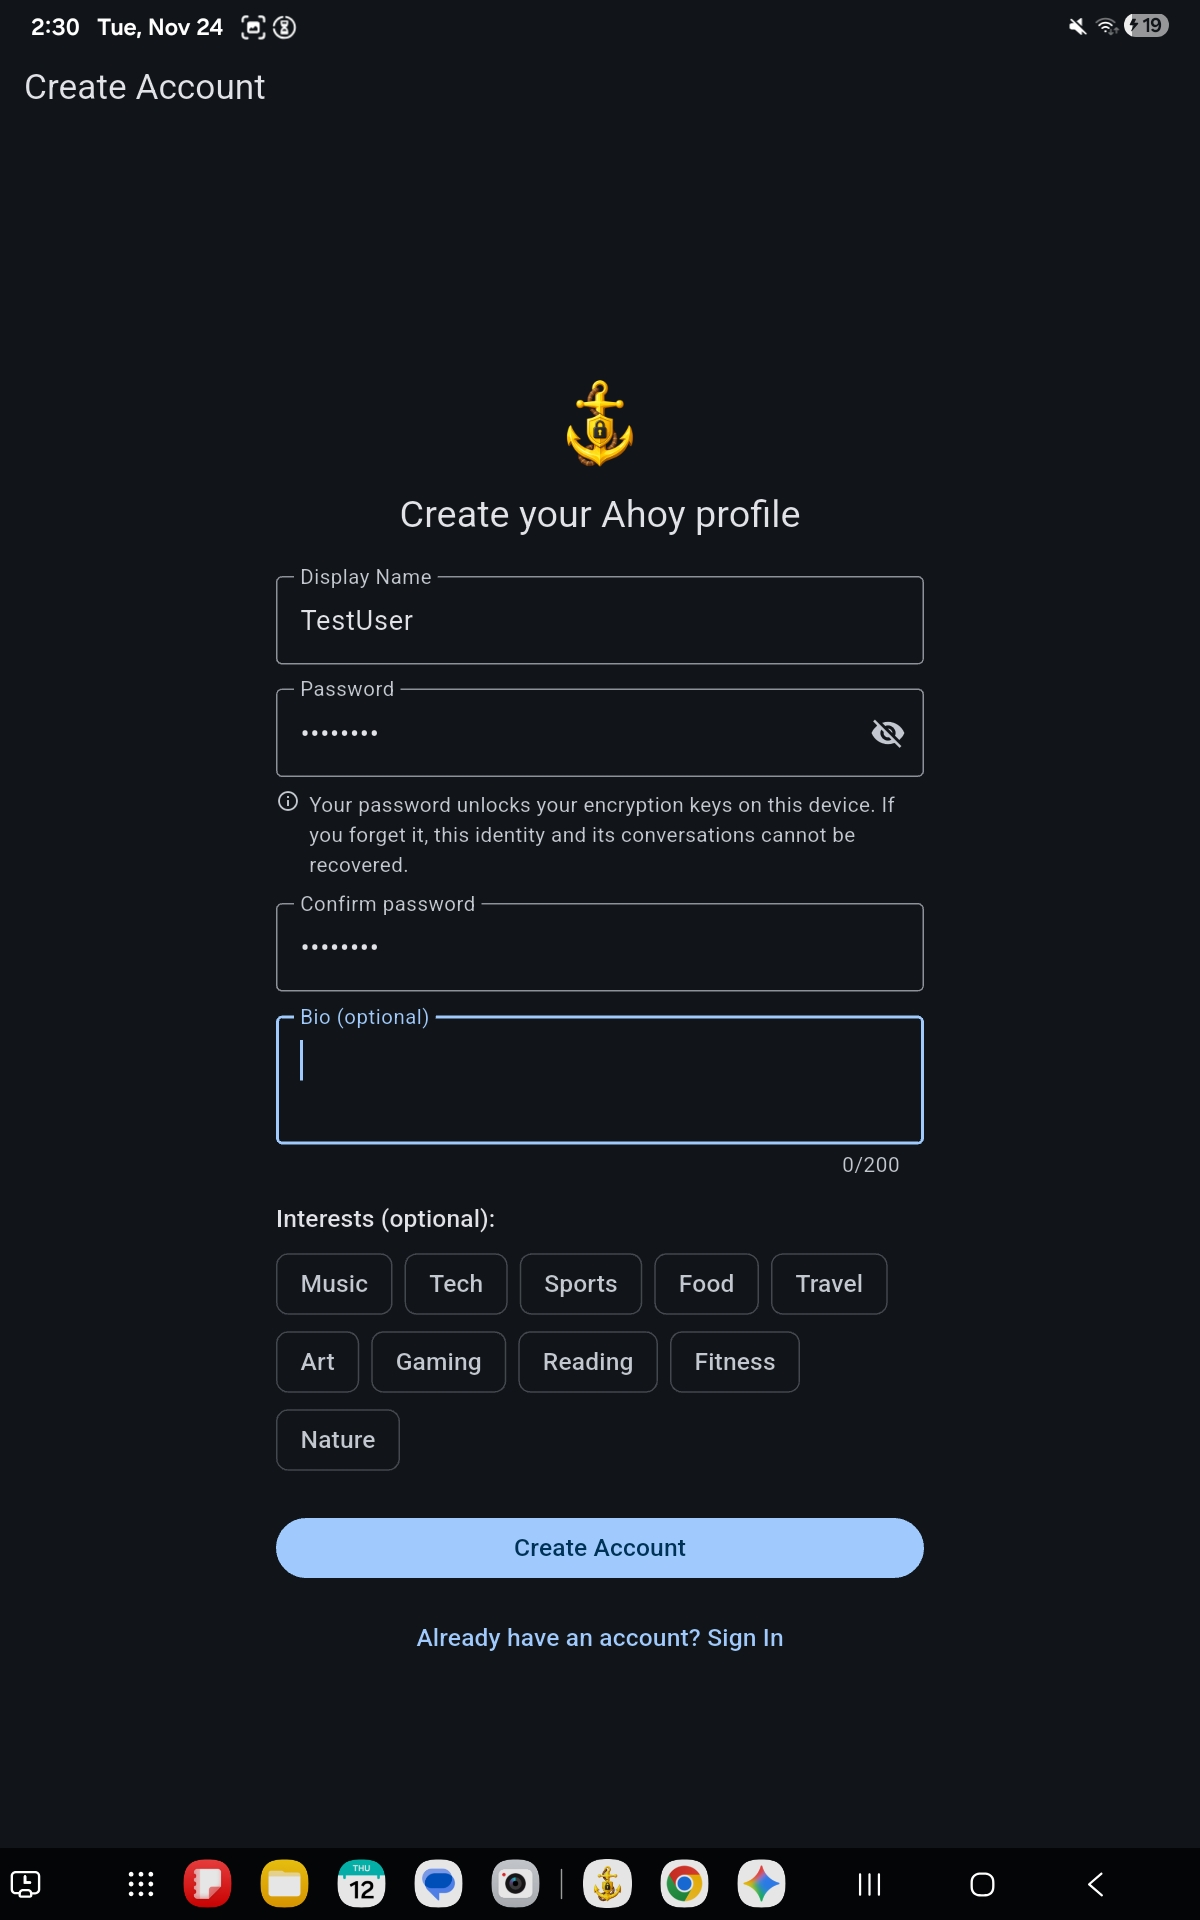
\includegraphics[width=0.175\linewidth]{img/ahoy-3.jpg}\hfill
  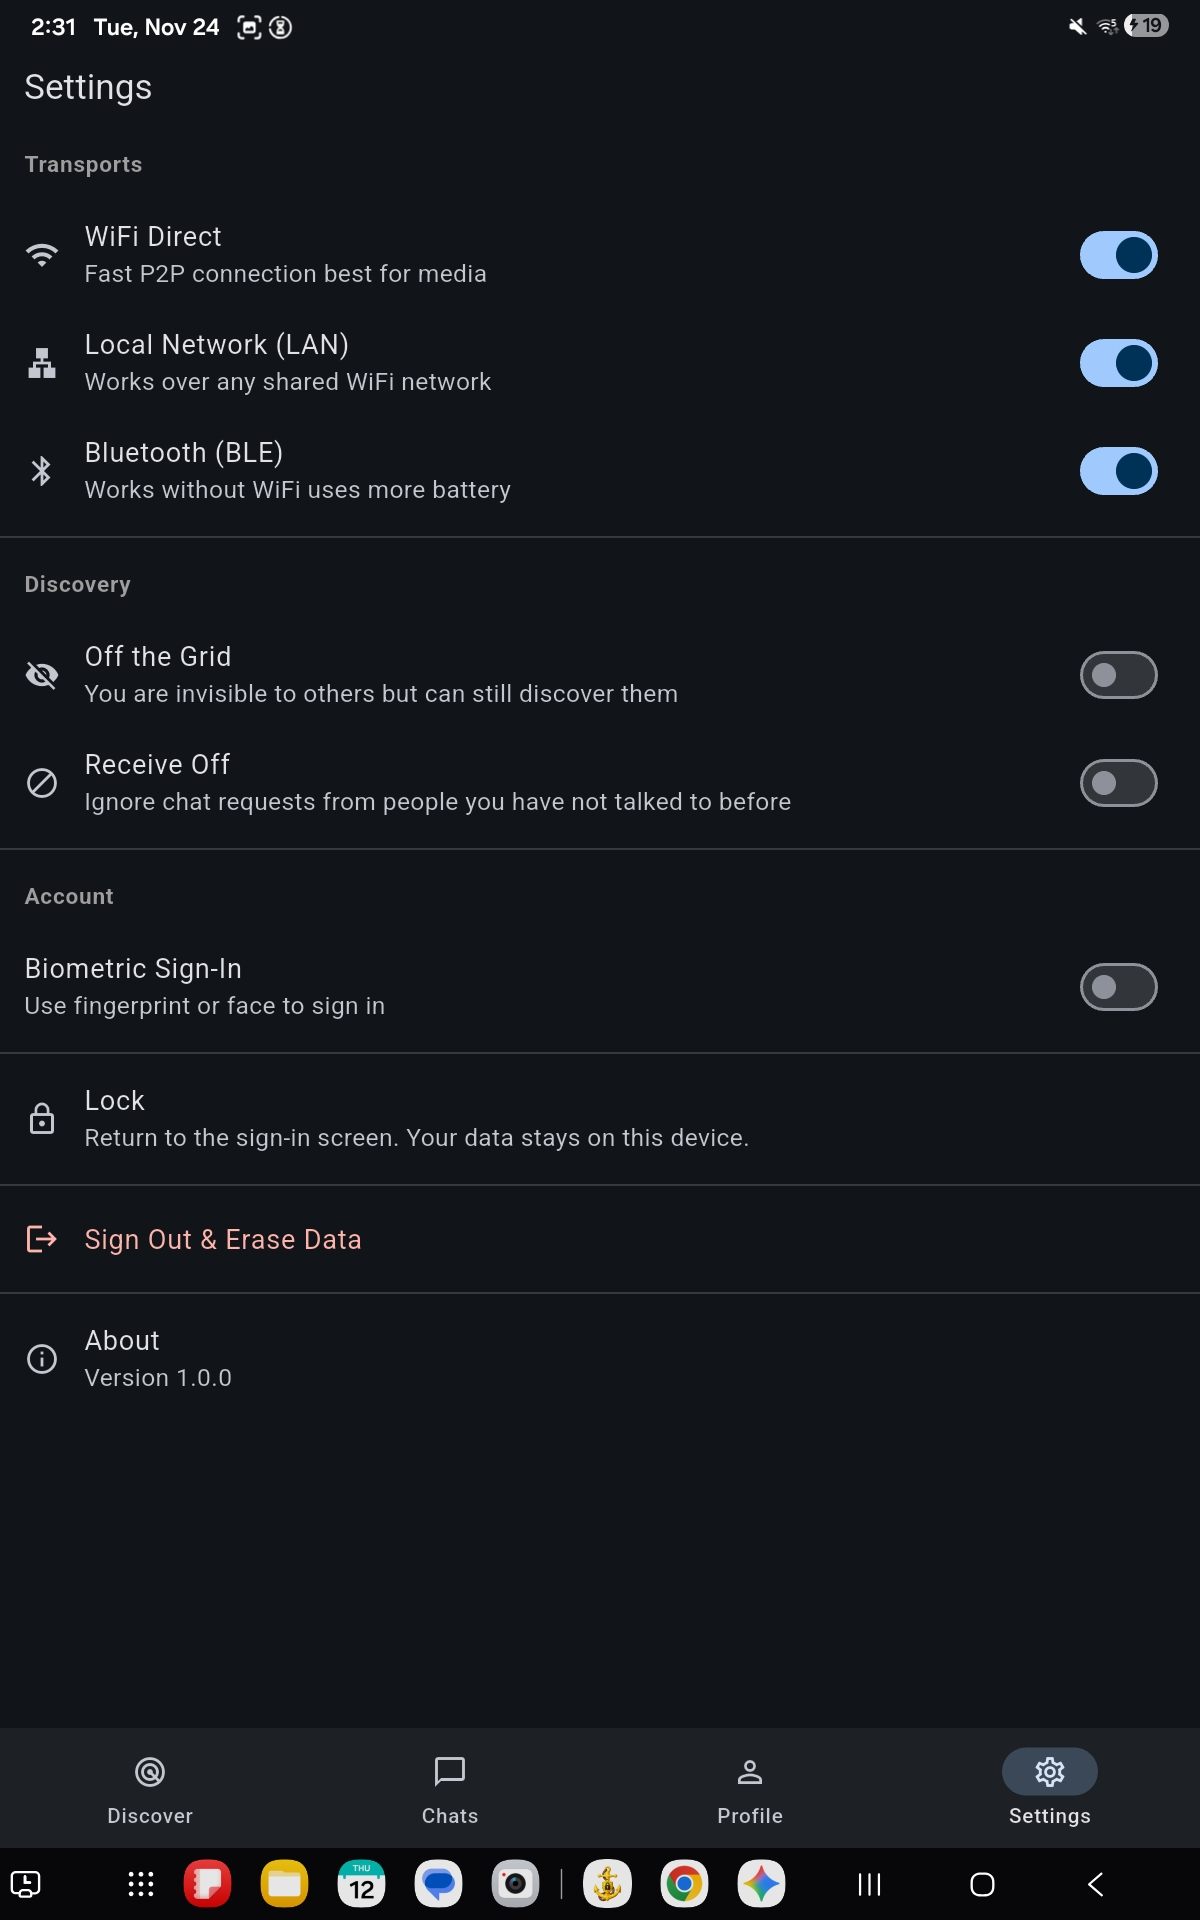
\includegraphics[width=0.175\linewidth]{img/ahoy-4.jpg}\hfill
  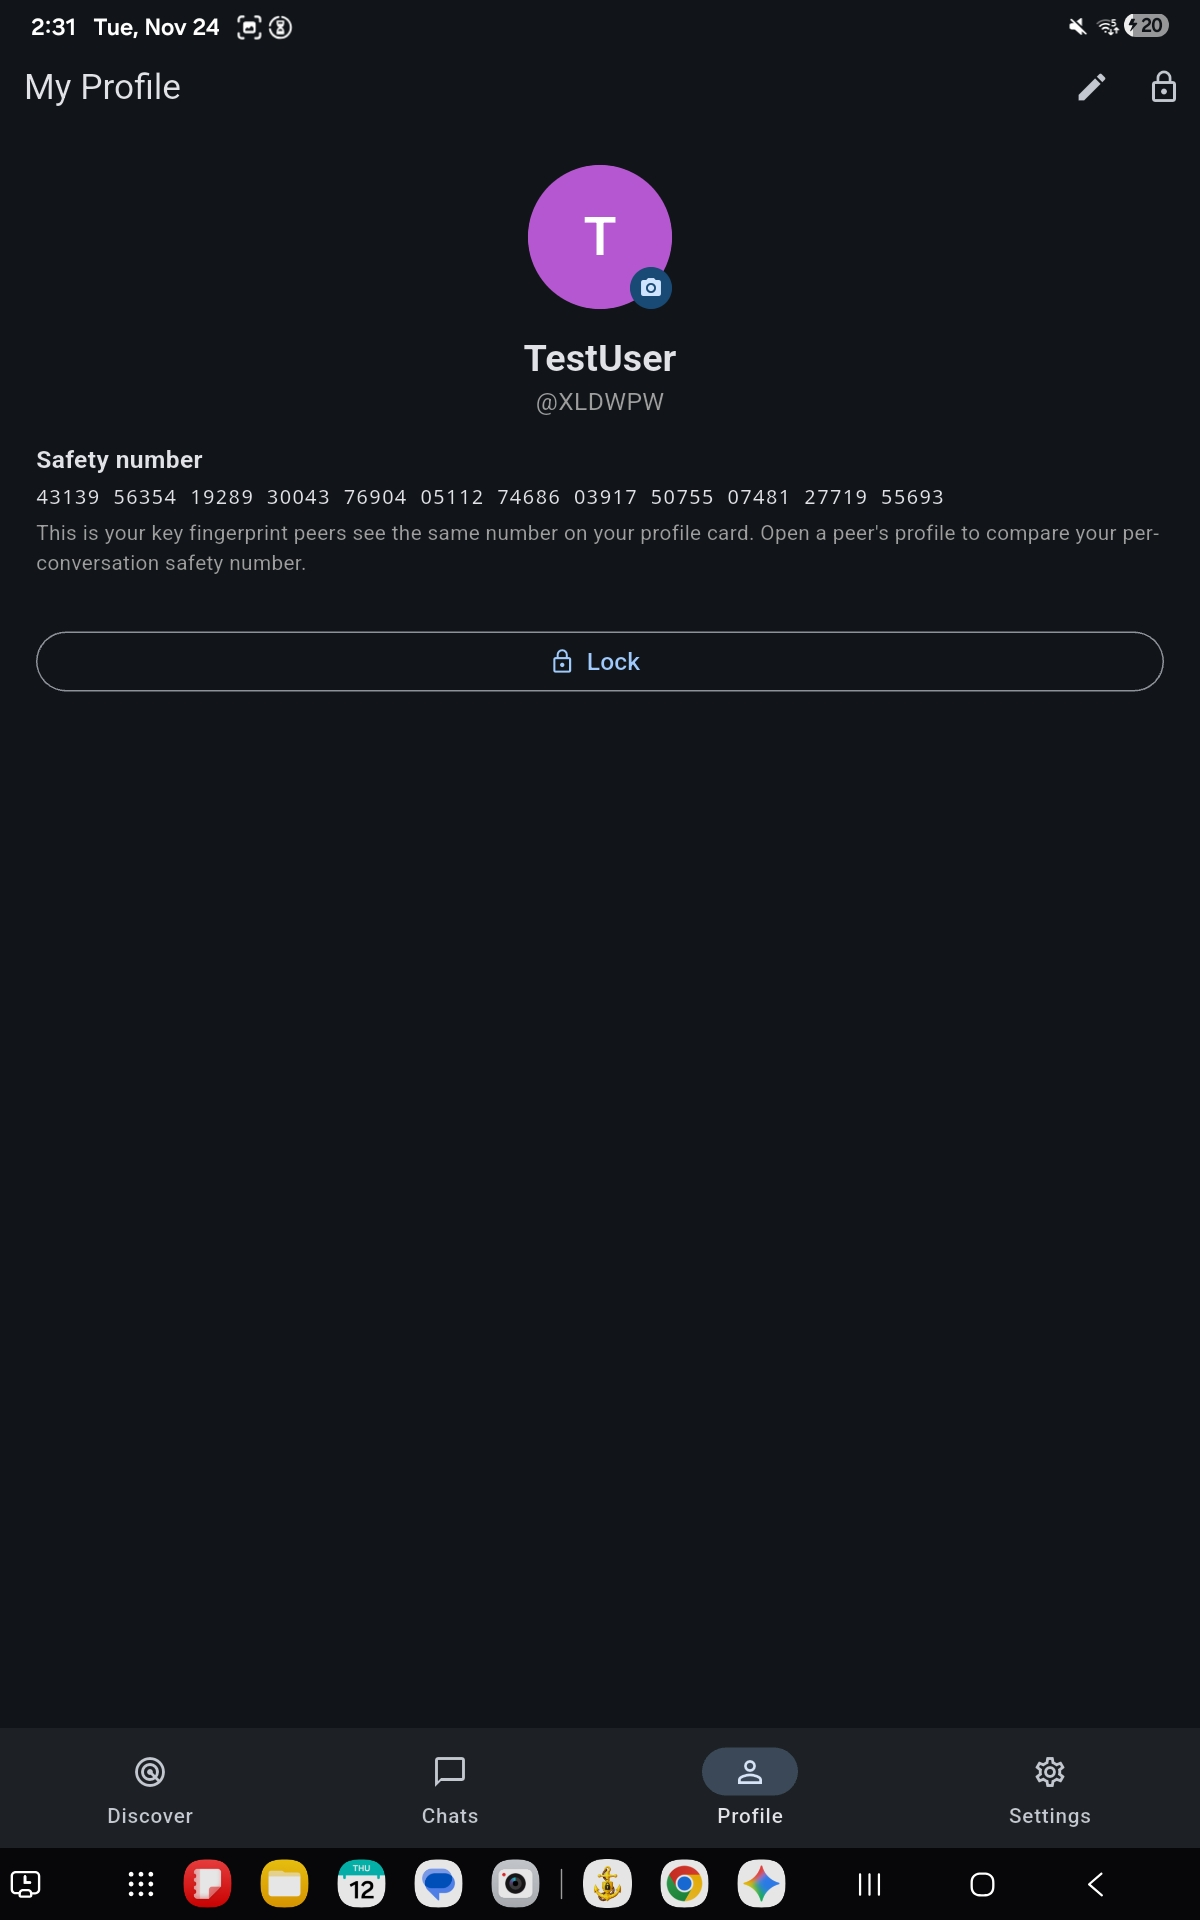
\includegraphics[width=0.175\linewidth]{img/ahoy-5.jpg}
\end{center}
\par\vspace{2pt}
\diag{img/mmd-ahoy.png}{0.95}

\end{proj}

%------------------------------------------------------------
\begin{proj}{Kalman GPS Tracking}{https://github.com/shamekhing/Kalman-Filter-for-GPS-Tracking}
A header-only C++ Kalman filter that turns jumpy GPS fixes into a smooth route.
It predicts where the vehicle should be, blends that with each GPS measurement,
and outputs a cleaned position and velocity track.

\vspace{5pt}
\stack{C++, Eigen, State estimation}
\shot{img/kalman.png}{0.85}
\diag{img/mmd-kalman.png}{0.95}

\end{proj}

%------------------------------------------------------------
\begin{proj}{Mean-Shift Clustering}{https://github.com/shamekhing/Mean-Shift-Clustering}
A mean-shift clustering implementation in C++ and Eigen. It groups 2-D points
without being told how many clusters exist, shifting each point toward its
neighborhood mean until they settle together.

\vspace{5pt}
\stack{C++, Eigen, Clustering}
\shot{img/mean-shift.png}{0.85}
\diag{img/mmd-mean-shift.png}{0.95}

\end{proj}

%------------------------------------------------------------
\begin{proj}{cooda}{https://github.com/shamekhing/cooda}
A complete 32-bit computer built from scratch in SystemVerilog: a 26-bit
instruction set, a 64 $\times$ 32-bit register file, a bit-serial ALU, and a bus
connecting BSRAM, DDR3 and an HDMI display. There is no vendor CPU core, and it
boots a handwritten-digit demo over HDMI.

\vspace{5pt}
\stack{SystemVerilog, Computer Architecture, FPGA}
\diag{img/mmd-cooda-datapath.png}{0.95}

\end{proj}

%------------------------------------------------------------
\begin{proj}{fpga-usb}{https://github.com/shamekhing/fpga-usb}
A USB CDC serial device implemented on a Gowin FPGA through an external ULPI PHY.
It turns the FPGA into a USB device a computer can talk to, with SystemVerilog
testbenches and host-side tools.

\vspace{5pt}
\stack{SystemVerilog, USB, FPGA}
\end{proj}

%------------------------------------------------------------
\begin{proj}{fpga-skill}{https://github.com/shamekhing/fpga-skill}
A reusable engineering workflow for Gowin FPGA projects, distilled from many
working sessions: one guide per task (RTL, simulation, synthesis, timing,
programming, debugging) plus tested scripts and checklists that stop steps being
skipped.

\vspace{5pt}
\stack{SystemVerilog, Gowin, Tooling}
\diag{img/mmd-fpga-skill.png}{0.95}

\end{proj}

%------------------------------------------------------------
\begin{proj}{pysuwi}{https://github.com/shamekhing/pysuwi}
A command-line toolbox with one rule: drop a Python file in the plugins folder
and it becomes a subcommand, with no registration needed. It ships with a pinned
installer and a doctor command that reports installation health.

\vspace{5pt}
\stack{Python, CLI, Tooling}
\diag{img/mmd-pysuwi.png}{0.95}

\end{proj}

\vspace{12pt}
{\color{accent}\rule{\linewidth}{0.9pt}}\\[4pt]
{\small\textbf{Contact}\quad
 \href{https://github.com/shamekhing}{GitHub} \textperiodcentered\
 \href{https://www.linkedin.com/in/shamekhalsuwi/}{LinkedIn} \textperiodcentered\
 \href{mailto:shamekhing@gmail.com}{shamekhing@gmail.com}}

\end{document}